\section{Part 1: Sequence Alignment}

The goal of sequence alignment is to find similarities between two sequences. These similarities might indicate homology, that is, highly similar sequences most likely share a common ancestor.

Alignments receive a score that measures how good they are.
In order to score alignments substitution matrices such as PAM or BLOSUM are used in combination with gap penalties.
When scoring alignments, lower numbers mean worse score, and higher numbers mean better score.

\subsection{Substitution Matrices}
\label{sec:substmats}

It is important to know how to obtain the alignment using substitution matrices, and how to obtain the substitution matrix from data. The data here come from trusted alignments which are known to be true from biology.

The substitution score is obtained by looking up the substitution matrix $s(x,y)$ for symbols $x_i$ and $y_j$.
Scores reflect how often we actually see a given substitution: substitutions that more often encountered, hence more likely to occur biologically, receive a higher score; conversely, rare substitutions receive a lower score.

The diagonal of the substitution matrix scores a match in position $(i,j)$ of the alignment, that is, $x_i = y_j$.
The diagonal does not always contain the same numbers, because some matches are more better than others: for instance if in trusted alignments we see more A-A
matches than C-C then the score of A-A in the diagonal of the substitution matrix will be higher than the score of C-C (meaning that seing an A-A match is more valuable than seing C-C).

In order to compute substitution scores we need to count the frequency of symbols (amino acids, nucleotides) and the frequency of their substitutions. Example for amino acids:
\begin{itemize}
\item $q_Q$: frequency of Q aminoacids
\item $p_{QR}$ frequency of Q $\leftrightarrow$ R substitutions
\end{itemize}

In general:
\begin{itemize}
\item $q_{x_i}$: frequency of symbol $x_i$ in trusted alignments
\item $p_{x_i, y_j}$ frequency of $x_i$ $\leftrightarrow$ $y_j$ substitutions in trusted alignments
\end{itemize}

%\begin{tabular}{lll}
%\item $q_Q$    & = & \% of Q aminoacids \\
%\item $p_{QR}$ & = & \% of Q $\leftrightarrow$ R substitutions
%\end{tabular}

Consider two aligned sequences $x$ and $y$ after dropping the gaps in their alignment:
\begin{itemize}
\item Probability of $x$ and $y$ when they are both random:
\begin{equation}
P(x, y|R) = P(x|R) p(y|R) = q_{x_1} q_{x_2} ... q_{y_1} q_{y_2} ... 
          = \prod_i q_{x_i} \prod_j q_{y_j}
\label{eq:probxyrnd}
\end{equation}
\item Probability of $x$ and $y$ when they are related:
\begin{equation}
P(x,y|M) = p_{x_1,y_1} p_{x_2,y_2} ... = \prod_i p_{x_i, y_i}
\label{eq:probxyrel}
\end{equation}
\end{itemize}

Compare equations (\ref{eq:probxyrel}) and (\ref{eq:probxyrnd}) using the {\bf odds ratio}, taking into account that after removing the gaps, the two sequences will have the same length:
\begin{equation}
\frac{P(x,y|M)}{P(x,y|R)} = 
\frac{\prod_i p_{x_i, y_i}}{\prod_i q_{x_i} \prod_j q_{y_j}} =
\prod_i \frac{p_{x_i, y_i}}{q_{x_i} q_{y_i}}
\label{eq:oddsratio}
\end{equation}

If $P(x,y|M) << P(x,y|R)$ then $x$ and $y$ are unrelated, else they are related.

The differences %(\textcolor{red}{in probability ???})
are usually huge, moreover computing the product in eq. (\ref{eq:oddsratio}) can lead to numerical problems, so it is better to take the logarithm of the odds ratio, resulting in the {\bf log-odds score}:
\begin{equation}
S(x,y) = 
\log \left( \frac{P(x,y|M)}{P(x,y|R)} \right) =
\log \left( \prod_i \frac{p_{x_i, y_i}}{q_{x_i} q_{y_i}} \right) =
\sum_i \log \left( \frac{p_{x_i, y_i}}{q_{x_i} q_{y_i}} \right)
\end{equation}

The quantity $S(x,y)$ is the total score for the alignment.
%behaves exactly like the substitution score.
It is the sum of the individual scores $s(a,b)$ for each pair of aligned symbols, which are looked up in the substitution matrix:
\begin{equation}
s(a,b) = \log \left( \frac{p_{ab}}{q_a q_b} \right)
\end{equation}

If two symbols are related (e.g. like the letters d-t, s-z, s-ss in Dutch vs. German), then the probability of seeing them together ($p_{ab}$) is higher than the probability of seeing them independently ($q_a q_b$):
%
\begin{itemize}
\item If $a$ and $b$ are {\bf related} then $p_{ab} > q_a q_b \Rightarrow \log(p_{ab}/(q_a q_b)) > 0 \Rightarrow$ {\bf positive score}
\item If $a$ and $b$ are {\bf unrelated} then $p_{ab} < q_a q_b \Rightarrow \log(p_{ab}/(q_a q_b)) < 0 \Rightarrow$ {\bf negative score}
\end{itemize}

Hence the substitution score measures the probability that the two amino acids are related (that is, often aligned) in reality.

%In substitution matrices, substitution scores are typically given as probabilities in log scale. Matrix scales such that the average value is zero: ...
% related to probab interpr of model
%matrix is symmetric, but doesn't have to 

\subsubsection{PAM and BLOSUM Matrices}

Two frequently used substitution matrices are PAM and BLOSUM:
\begin{itemize}
%
\item Point Accepted Mutations (PAM): \\
PAM1 matrix: 1\% point accepted mutations \\
PAM250 is 250\% point accepted mutations ($\approx$ 20\% similarity): PAM1 to the power 250. \\
Beware that PAM doesn't work well for large evolutionary distances. 
%
\item BLOSUM matrix (BLOCKS SUbstitution): \\
Computed from ungapped alignments in the BLOCKS database, which is a db of validated alignments. \\
The number of the BLOSUM matrix (e.g. BLOSUM80, BLOSUM62, BLOSUM50) is the maximum percentage of similarity used in the construction of the matrix.
%
\end{itemize}

The PAM matrix tries to turn the evolutionary clock back in time by trying to bring sequences to the situation where there's only 1\% differences between them.
If two sequences are close (e.g. human vs chimp), the evolutionary clock will turn back only a little.
% ly: PAM distance is short. ???
Conversely, if two sequences are distant (e.g. human vs yeast), then the evolutionary clock must turn back a lot in order to get to the point where there was only 1 \% difference between them.

%https://en.wikipedia.org/wiki/BLOSUM
A BLOSUM\{L\} matrix results from the comparison between sequences that have {\em at most} L\% similarity: those sequences that have more than L\% identical amino acids are grouped together in one cluster and considered as a single sequence: all the sequences that are sufficiently different (belonging to different clusters) are then aligned together and the score put in the BLOSUM\{L\}  matrix. 

A BLOSUM matrix with high L (e.g. BLOSUM80) is appropriate to align closely related sequences, such as mouse and human (with short evolutionary distance hence high similarity). Conversely, low L is suitable to align distant sequences such as human and yeast (low similarity). An intermediate matrix such as BLOSUM62 is appropriate to score sequences that are not so close, not so far, such as human and chicken.

\subsection{Gap Penalties: Opening Gaps vs. Extension Gaps}

The gap penalty penalizes for gaps in the alignment. It is typically a negative number: $G = - d < 0$ for a gap in one position. The lower the  number the more severe the penalty (it makes the score of the alignment decrease).

{\bf Opening gap} vs. {\bf extension gap} penalty: sometimes a whole piece is missing in a sequence, but we don't want the penalty to be too big for it, just skip missing piece and go on. So the 2nd gap (extension gap) is usually cheaper (less severe penalty) than the 1st gap (opening gap):
\begin{verbatim}
e.g. -8 penalty for 1st gap (= opening gap)
     -4 penalty for 2nd gap (= extension gap)
\end{verbatim}

\subsection{Shortest Path with Dynamic Programming}

Dynamic programming is used to solve the shortest path problem, e.g. finding shortest path between 2 cities (like GPS navigator), see \ref{fig:shortestpath}. It is based on {\bf Belman's optimality principle}: if I have the shortest path (optimal), then any subpath must be optimal too: there cannot be a shortcut in the optimal path, otherwise it wouldn't be the optimum!

\begin{figure}[!htb]
\centerline{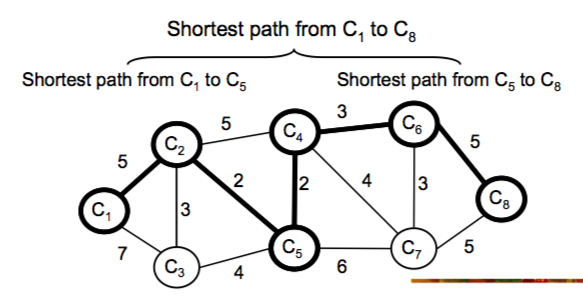
\includegraphics[width=.6\linewidth]{figs/shortestpath.png}}
\caption{Solving the shortest path problem}\label{fig:shortestpath}
\end{figure}

For instance, in figure \ref{fig:shortestpath}, either C6 or C7 is in the shortest path to C8. So if I know the shortest path to C6 or to C7, then I know which one is on the shortest path to C8.

\begin{verbatim}
e.g. if C1-C6 = 12
        C1-C7 = 13
      then C1-C6-C8 = 12+5 = 17 better (choose this one)
           C1-C7-C8 = 13+5 = 18 worse (discard)
best way to reach C6:
C1-C4 = 9 ==> C1-C4-C6 = 9 + 3 = 12
C1-C5 = 7 ==> C1-C5-C7 = 7 + 6 = 13
etc.
\end{verbatim}

\subsection{Global Alignment: Needleman-Wunsch Algorithm}

Given two sequences $x=x_1,...,x_i,...$ and $y=y_1,...,y_j,...$ to align (or {\em query} and {\em target}), make a matrix $F$ of the alignment, with one sequence in the rows and the other in the columns, plus one starting position (0,0) at the top left corner. Initially the matrix is empty, as shown in figure \ref{fig:fijempty}. We will fill in the matrix $F$ such that position $(i,j)$ gives the score $F(i,j)$ of the best alignent up to this position (with higher numbers meaning better score).

\begin{figure}[!htb]
\centerline{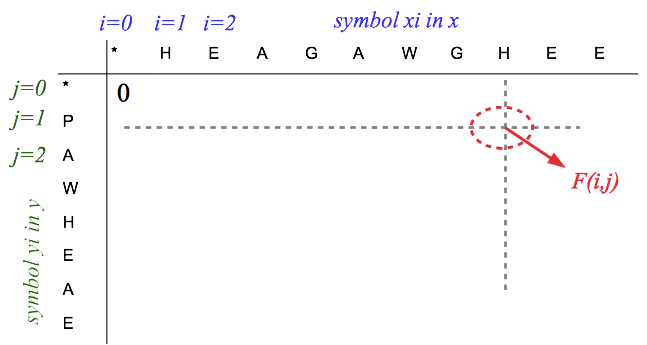
\includegraphics[width=.6\linewidth]{figs/fijempty.png}}
\caption{Initial state of matrix $F$ of the alignment.}\label{fig:fijempty}
\end{figure}

\textcolor{red}{IMPORTANT!! The convention here is that $i$ is the {\bf column} and $j$ is the {\bf row} of matrix $F$ !!! Hence the first sequence $x$ is placed horizontally (one symbol per column), and the second sequence $y$ is placed vertically (one symbol per row).}

An alignment can be seen as a particular path through the matrix of the alignment. The problem of finding the best alignment is then the problem of finding the legal path with the highest score, using only 3 legal movements through the matrix: diagonally down, right or down. This is analogous to the shortest path problem, and can be solved by dynamic programming.

Legal movements:
\begin{itemize}
\item Diagonally down = from $(i-1, j-1)$ to $(i,j)$:
using substitution score $S(x_i, y_j)$
%
\item Right or Down using gap score:
  \begin{itemize}
%
  \item Vertically {\bf down} = from $j-1$ to $j$: {\bf insertion} \textcolor{blue}{in the second strand} \\
\textcolor{red}{we move down, hence in the direction of the second strand ($x$) whereas the 1st strand ($x$) gets stalled (hence we put a gap in the first one, so there's an insertion in the second one)}
%
  \item Horizontally to the {\bf right} = from $i-1$ to $i$: {\bf deletion} \textcolor{blue}{in the second strand}\\
\textcolor{red}{we move right, hence in the direction of the first strand ($x$) whereas the 2nd strand ($y$) gets stalled (hence we put a gap there, meaning that the symbol is deleted from the 2nd one)}
%
  \end{itemize}
\end{itemize}

How to fill in the matrix: start from the top left corner $F(0,0)=0$, then complete each column successively computing the alignment score $F(i,j)$ as the best of 3 possible scores:

%\begin{equation}
%\begin{aligned}
%& F(i-1, \; j-1) + s(x_i, y_j) & 
%\quad \text{going diagonally using subst. score} \quad s() \\
%F(i,j) = \max \quad \quad
%& F(i, \; j-1) - d   & \quad \text{gap penalty:} \quad G = - d \\
%& F(i-1, \; j) - d   & \quad \text{gap penalty} &
%\nonumber
%\end{aligned}
%\label{eq:align:maxf}
%\end{equation}

\vskip 1em
\begin{tabular}{|lll|}
\hline
Substitution: & $S = F(i-1, \; j-1) + s(x_i, y_j)$ & 
  move diagonally using subst. score $s()$ \\
Insertion: & $D = F(i, \; j-1) - d$   & 
  move down using gap penalty: $G = - d$ \\
Deletion: & $I = F(i-1, \; j) - d$  &
  move right using gap penalty \\
Score: & $F(i,j) = \max(S, I, D)$ & maximum of the 3 possibilities above \\
\hline
\end{tabular}
\vskip 1em

This is shown in Figure \ref{fig:maxfij}.

\begin{figure}[!htb]
\centerline{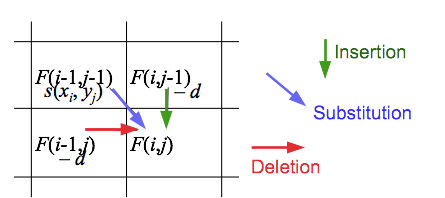
\includegraphics[width=.5\linewidth]{figs/maxfij.png}}
\caption{How to fill in the matrix $F$ of the alignment.}\label{fig:maxfij}
\end{figure}

An example of resulting matrix $F$ after filling in all the positions is shown in figure \ref{fig:fijfilled}

\begin{figure}[!htb]
\centerline{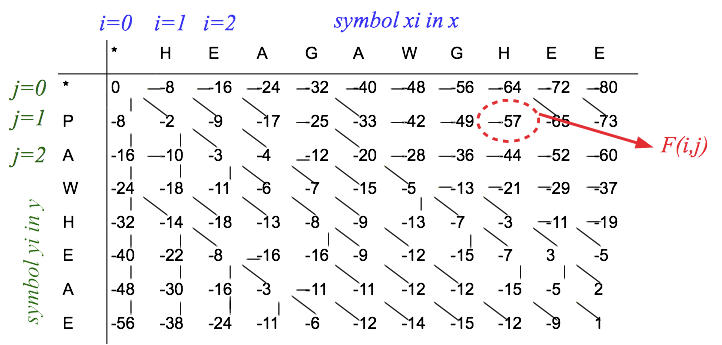
\includegraphics[width=.8\linewidth]{figs/fijfilled.png}}
\caption{Example of filled matrix $F$.}\label{fig:fijfilled}
\end{figure}

An alignment can be seen as a particular path through the matrix, following the best path found in the maximization procedure above. In order to determine the best global alignment, look at the last position of $F$ (bottom right slot), and  retrace the maximization steps back to the first position $(0,0)$, building position $k$ of the alignment $a_x,a_y$ at each step:
\begin{itemize}
\item if the optimum at position $(i,j)$ was a substitution, put align symbol $x_i$ and symbol $y_j$ on top of each other, and move to position $(i-1, j-1)$.
\item if the optimum was an insertion (vertical bar) then $a_{xk}=$ '-' (gap) and $a_{yk}=y_j$; move upwards to position $(i, j-1)$.
\item if the optimum was a deletion (horizontal bar) then $a_{xk}=x_i$ $a_{yk}=$ '-' (gap); move left to position $(i-1, j)$.
\item Decrement $k$ and repeat this until we reach $F(0,0)=0$.
\end{itemize}

Figure \ref{fig:traceback} shows an example of global alignment resulting from this procedure.
\\
\textcolor{red}{Note that the gap scores of this matrix do not match those of figure \ref{fig:fijfilled}. Probably an extension penalty of zero was applied!?!?!?}

\begin{figure}[!htb]
\centerline{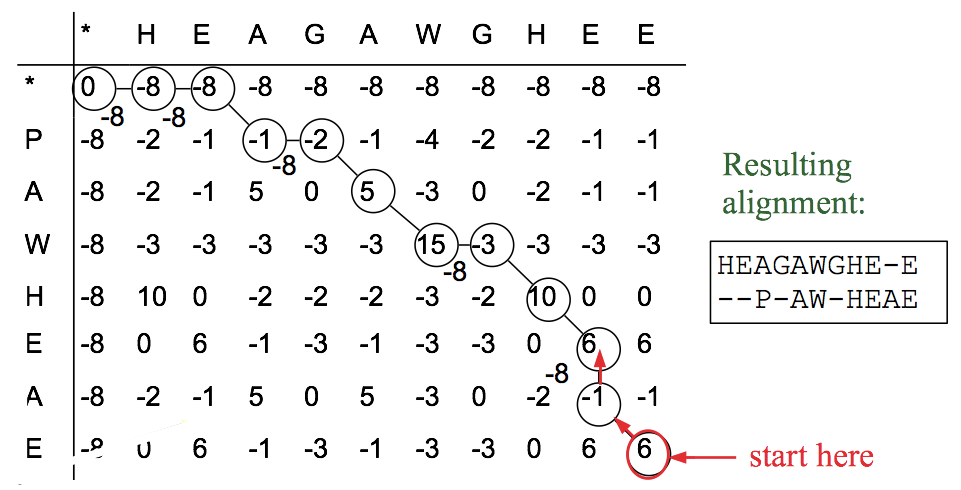
\includegraphics[width=.8\linewidth]{figs/traceback.png}}
\caption{Finding the optimum global alignment by tracing matrix $F$ from the bottom-right position back to $(0,0)$.}\label{fig:traceback}
\end{figure}

\subsection{Local Alignment: Smith-Waterman Algorithm}

The goal of a local alignment algorithm is to find the best matching subsequence between two sequences. The algorithm is similar to the global alignment, with two phases: fill in the $F$ matrix one by one (from left-top to right-down), then traceback following the pointers to the maximum scores. Except that now negative scores get reset to zero when filling in $F$, and we start from the highest score (and not from the bottom-right position) when tracing back.

This is the procedure to fill in the $F$ matrix:
\vskip 1em
\begin{tabular}{|lll|}
\hline
Initialization: & $F(0,0)=0$ & \\
\hline
Substitution: & $S = F(i-1, \; j-1) + s(x_i, y_j)$ & 
  move diagonally using subst. score $s()$ \\
Insertion: & $D = F(i, \; j-1) - d$   & 
  move down using gap penalty: $G = - d$ \\
Deletion: & $I = F(i-1, \; j) - d$  &
  move right using gap penalty \\
Restart: & $R=0$ & \\
Score: & $F(i,j) = \max(S, I, D, R)$ & maximum of the 4 possibilities above \\
\hline
\end{tabular}
\vskip 1em

The procedure to trace back and find the local alignment is shown in figure \ref{fig:traceback-local} using an example.

\begin{figure}[!htb]
\centerline{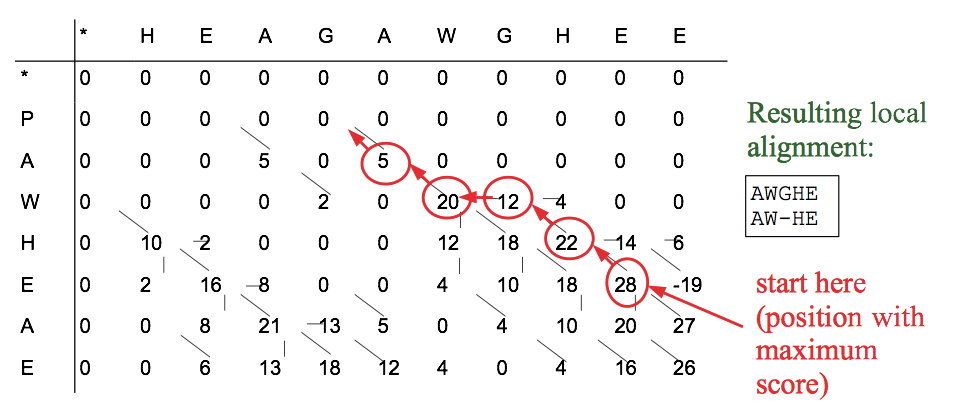
\includegraphics[width=.8\linewidth]{figs/traceback-local.png}}
\caption{Example of finding the optimum local alignment by tracing back matrix $F$ from the position with highest score back to the position where the score becomes zero.}\label{fig:traceback-local}
\end{figure}

Both local and global alignment algorithms have quadratic complexity.

\subsection{Statistical Significance of Alignments}

Once we have a score for our alignment, how to judge if this score good or bad? How to assess if an alignment is good or bad? Answer: we must assess its statistical signifcance, hence compute its p-value. A small p-value means that the alignment is significantly better than what can be expected by random chance.

The computation of the p-value of an alignment relies on the fact that the score of a pair random sequences is normally distributed: if we pick two random sequences, align them, get the score, then repeat this many many times, the set of scores obtained is normally distributed. So a statistically significant score must do a lot better than this normal distribution. How much better? Better than most of the best random scores. For this we must look at the distribution of maximum scores out of a set of random scores.

The maximum of a set of normally distributed values (scores of random sequences in our case) follows the Extreme Value Distribution (EVD). A significantly good alignment must have a score that is much larger than most of the best random scores, which are EVD distributed. That is, the score for a good alignment should lie at the extreme right tail of the EVD distribution. This is explained in more detail below.

\subsubsection{Extreme Value Distribution (EVD)}

If I repeat the following procedure several times:
\begin{itemize}
\item draw $n$ samples from a normal distribution
\item take the maximum $M_n$ of these $n$ samples
\end{itemize}
then the probability that the maximum $M_n$ is within a specified value $x$ follows the {\bf extreme value distribution (EVD)}:
%
\begin{equation}
P(M_N \le x) = \exp(- K \; n \; e^{\lambda(x - \mu)} )
\label{eq:evd}
\end{equation}
\textcolor{red}{this is an exponential of an exponential!!}

Figure \ref{fig:evd-unscaled} shows the shape of the unscaled EVD, for $\lambda=1$, $\mu =0$, and $Kn= 1$.

\begin{figure}[!htb]
\centerline{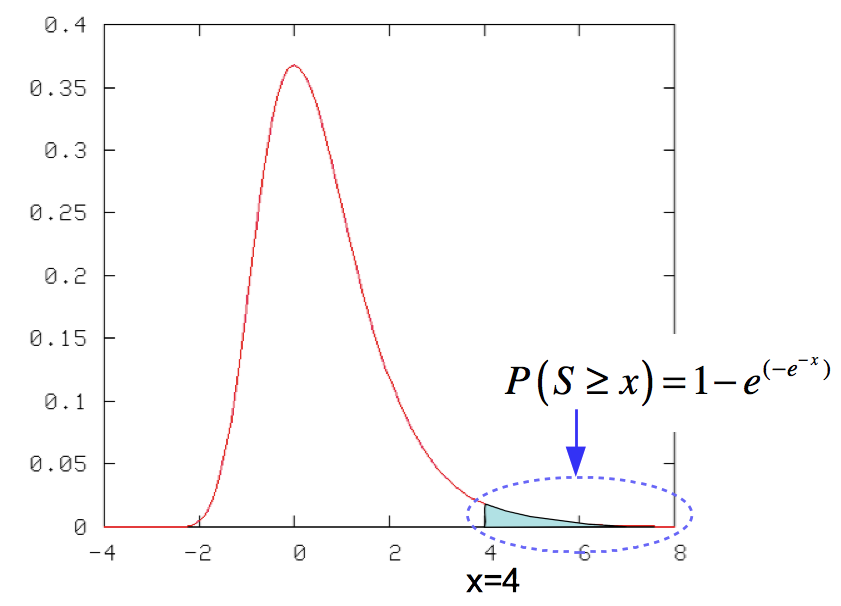
\includegraphics[width=.6\linewidth]{figs/evd-unscaled.png}}
\caption{Extreme Value Distribution, unscaled. For an alignment to be significant, the shaded area under the curve should be sufficiently small.
From \url{http://elbo.gs.washington.edu/courses/GS\_373\_12\_sp/slides/6A-significance\_scores.pdf}}
\label{fig:evd-unscaled}
\end{figure}

For ungapped alignments, the EVD has the form of 
eq. (\ref{eq:evd}). For gapped alignments, the EVD has the extended form:
\begin{equation}
P(S \le x) = \exp(- K \; n \; m \; e^{- \lambda x} )
\label{eq:evdgap}
\end{equation}
where $n$ is the length of the query, and $m$ is sum of the lengths of all sequences in the target database.

%Note that $m n$ can be a huge number, but ok, because it's like winning the lottery if many people are playing: someone is likely to win.
%The size of the db will decrease your significance score: like lottery.

%LY: so why isn't m also in the formula without gaps? (sl. 28)
%prof: because in this case K encompases m too (more general formula)

\subsubsection{Assessing Scores Based on the EVD}

How high my score has to get to make sure it doesn't come from the normal distribution of random scores? It must be better than the best random alignments among a large number of sequences.

%e-value: score: alignment is significant if its score is less than $1\%$.

Let $x$ be the score of my alignment. If the probability of getting a maximum score $S$ better than my score $x$ is sufficiently small, say, less than $1 \%$, then my alignment is significant:

If $P(S > x) = 1 - P(S \le x) < 0.01$ then the alignment is significant. \\
where $ P(S \le x)$ is calculated according to eq. (\ref{eq:evdgap}).

\subsection{BLAST}

BLAST is used to search for a sequence in a database of sequences. The sequence we're looking for is called the {\em query} and the sequences stored in the database are the {\em targets}. Due to the huge number of target sequences, Smith-Waterman local alignment would be too slow, so a more efficient algorithm is needed.

Basic Local Alignment Search Tool (BLAST) solves this problem using heuristics. It works by performing a fast and cheap search at the beginning,
that allows us to eliminate most of the non-promising targets, and then focusing on the fewer potentially promising hits for closer inspection.

Steps of the BLAST algorithm:
\begin{itemize}
\item {\bf Step 1: look for triplets} \\
  This step is cheap, computationally.
  Given a query such as 'RNQHEEWAPRDCNRH':
  \begin{itemize}
  \item look up all the triplets in this sequence: RNQ, NQH, QHE, ..., etc. in potential targets;
  \item also include triplets that are not in the query but are similar enough: \\
    RNQ: RNE, RNH, RQQ ... \\
    NQH: NHQ, NHA, NRH, ...
  \item make a tree out of all the triplets:
\begin{verbatim}
R -> N -> Q
       -> E
       -> H
  -> Q -> Q
       -> E
N -> R -> H
       -> Q
  -> Q -> W
       -> A
       -> H
\end{verbatim}
  \end{itemize}
\item {\bf Step 2: regular expression search}
  \begin{itemize}
  \item Use a regular expression algorithm (finite state automaton) to perform the search for the triplets in the db.
  \item Keep track of the match position in query and target.
  \item The score doesn't matter much at this point, and doesn't depend on the number of matching triplets: if the same triplet is found several times, or multiple triples found in targets, the score is not higher, just mark all the targets that match.
  \end{itemize}

\item {\bf Step 3: select pairs of closeby hits}
  \begin{itemize}
  \item take 2 triplet hits next to each other (or very close): \\
  assume subblock without gaps with 2 matching hits, in order to avoid dynamic programming
(this might miss a good alignment but with lots of gaps, but we hope it doesn't occur too ofen)
  \item discard targets with no 2 hits
  \end{itemize}

\item {\bf Step 4: extend without gaps}
  \begin{itemize}
  \item for each block found in step 3, try to extend the block in both directions (left and right), see if still matches nicely:
%
\begin{verbatim}
NQHEEWAPRDCNRH
NRHWWWRPRNCANR
       ++-+---

+ : increase score
- : decrease score
\end{verbatim}

  \item score goes up with a match, down with mismatch (remember that no gaps are considered at this stage)
  \item keep the highest score that you've been able to extend without gaps 
        ({\em high scoring segment pair} ({\bf HSP}))
  \item extend further until the score decreases too much
% can't rescue anymore
%this gives us a gap extension
  \end{itemize}

\item {\bf Step 5: extend HSPs with gaps}
  \begin{itemize}
  \item extend the HSPs by gapped alignment
  \item stop the extension when the score drops by $X_g$ (e.g., $X_g$=40) under the best score so far;
  \item select the best gapped local alignment
  \end{itemize}

\item {\bf Step 6: assess significance}
  \begin{itemize}
  \item compute the statistical significance of the alignments (hits);
  \item for the significant alignments, repeat the gapped alignment (step 5) with a higher dropoff parameter $X_g$ for more accuracy.
  \end{itemize}

\end{itemize}



%---------------------------------------------------------------------------

